\documentclass[a4paper,twoside]{article}
% My LaTeX preamble file - by Nathaniel Dene Hoffman
% Credit for much of this goes to Olivier Pieters (https://olivierpieters.be/tags/latex)
% and Gilles Castel (https://castel.dev)
% There are still some things to be done:
% 1. Update math commands using mathtools package (remove ddfrac command and just override)
% 2. Maybe abbreviate \imath somehow?
% 3. Possibly format for margin notes and set new margin sizes
% First, some encoding packages and useful formatting
%--------------------------------------------------------------------------------------------
\usepackage{import}
\usepackage{pdfpages}
\usepackage{transparent}
\usepackage[l2tabu,orthodox]{nag}   % force newer (and safer) LaTeX commands
\usepackage[utf8]{inputenc}         % set character set to support some UTF-8
                                    %   (unicode). Do NOT use this with
                                    %   XeTeX/LuaTeX!
\usepackage[T1]{fontenc}
\usepackage[english]{babel}         % multi-language support
\usepackage{sectsty}                % allow redefinition of section command formatting
\usepackage{tabularx}               % more table options
\usepackage{booktabs}
\usepackage{titling}                % allow redefinition of title formatting
\usepackage{imakeidx}               % create and index of words
\usepackage{xcolor}                 % more colour options
\usepackage{enumitem}               % more list formatting options
\usepackage{tocloft}                % redefine table of contents, new list like objects
\usepackage{subfiles}               % allow for multifile documents

% Next, let's deal with the whitespaces and margins
%--------------------------------------------------------------------------------------------
\usepackage[centering,margin=1in]{geometry}
\setlength{\parindent}{0cm}
\setlength{\parskip}{2ex plus 0.5ex minus 0.2ex} % whitespace between paragraphs

% Redefine \maketitle command with nicer formatting
%--------------------------------------------------------------------------------------------
\pretitle{
  \begin{flushright}         % align text to right
    \fontsize{40}{60}        % set font size and whitespace
    \usefont{OT1}{phv}{b}{n} % change the font to bold (b), normally shaped (n)
                             %   Helvetica (phv)
    \selectfont              % force LaTeX to search for metric in its mapping
                             %   corresponding to the above font size definition
}
\posttitle{
  \par                       % end paragraph
  \end{flushright}           % end right align
  \vskip 0.5em               % add vertical spacing of 0.5em
}
\preauthor{
  \begin{flushright}
    \large                   % font size
    \lineskip 0.5em          % inter line spacing
    \usefont{OT1}{phv}{m}{n}
}
\postauthor{
  \par
  \end{flushright}
}
\predate{
  \begin{flushright}
  \large
  \lineskip 0.5em
  \usefont{OT1}{phv}{m}{n}
}
\postdate{
  \par
  \end{flushright}
}

% Mathematics Packages
\usepackage[Gray,squaren,thinqspace,cdot]{SIunits}      % elegant units
\usepackage{amsmath}                                    % extensive math options
\usepackage{amsfonts}                                   % special math fonts
\usepackage{mathtools}                                  % useful formatting commands
\usepackage{amsthm}                                     % useful commands for building theorem environments
\usepackage{amssymb}                                    % lots of special math symbols
\usepackage{mathrsfs}                                   % fancy scripts letters
\usepackage{cancel}                                     % cancel lines in math
\usepackage{esint}                                      % fancy integral symbols
\usepackage{relsize}                                    % make math things bigger or smaller
%\usepackage{bm}                                         % bold math!
\usepackage{slashed}

\newcommand\ddfrac[2]{\frac{\displaystyle #1}{\displaystyle #2}}    % elegant fraction formatting
\allowdisplaybreaks[1]                                              % allow align environments to break on pages

% Ensure numbering is section-specific
%--------------------------------------------------------------------------------------------
\numberwithin{equation}{section}
\numberwithin{figure}{section}
\numberwithin{table}{section}

% Citations, references, and annotations
%--------------------------------------------------------------------------------------------
\usepackage[small,bf,hang]{caption}        % captions
\usepackage{subcaption}                    % adds subfigure & subcaption
\usepackage{sidecap}                       % adds side captions
\usepackage{hyperref}                      % add hyperlinks to references
\usepackage[noabbrev,nameinlink]{cleveref} % better references than default \ref
\usepackage{autonum}                       % only number referenced equations
\usepackage{url}                           % urls
\usepackage{cite}                          % well formed numeric citations
% format hyperlinks
\colorlet{linkcolour}{black}
\colorlet{urlcolour}{blue}
\hypersetup{colorlinks=true,
            linkcolor=linkcolour,
            citecolor=linkcolour,
            urlcolor=urlcolour}

% Plotting and Figures
%--------------------------------------------------------------------------------------------
\usepackage{tikz}          % advanced vector graphics
\usepackage{pgfplots}      % data plotting
\usepackage{pgfplotstable} % table plotting
\usepackage{placeins}      % display floats in correct sections
\usepackage{graphicx}      % include external graphics
\usepackage{longtable}     % process long tables

% use most recent version of pgfplots
\pgfplotsset{compat=newest}

% Misc.
%--------------------------------------------------------------------------------------------
\usepackage{todonotes}  % add to do notes
\usepackage{epstopdf}   % process eps-images
\usepackage{float}      % floats
\usepackage{stmaryrd}   % some more nice symbols
\usepackage{emptypage}  % suppress page numbers on empty pages
\usepackage{multicol}   % use this for creating pages with multiple columns
\usepackage{etoolbox}   % adds tags for environment endings
\usepackage{tcolorbox}  % pretty colored boxes!


% Custom Commands
%--------------------------------------------------------------------------------------------
\newcommand\hr{\noindent\rule[0.5ex]{\linewidth}{0.5pt}}                % horizontal line
\newcommand\N{\ensuremath{\mathbb{N}}}                                  % blackboard set characters
\newcommand\R{\ensuremath{\mathbb{R}}}
\newcommand\Z{\ensuremath{\mathbb{Z}}}
\newcommand\Q{\ensuremath{\mathbb{Q}}}
%\newcommand\C{\ensuremath{\mathbb{C}}}
\renewcommand{\arraystretch}{1.2}                                       % More space between table rows (could be 1.3)
\newcommand{\Cov}{\mathrm{Cov}}
\newcommand\D{\mathrm{D}}
\newcommand*{\dbar}{\ensuremath{\text{\dj}}}

\newcommand{\incfig}[2][1]{%
    \def\svgwidth{#1\columnwidth}
    \import{./figures/}{#2.pdf_tex}
}

% Custom Environments
%--------------------------------------------------------------------------------------------
\newcommand{\lecture}[3]{\hr\\{\centering{\large\textsc{Lecture #1: #3}}\\#2\\}\hr\markboth{Lecture #1: #3}{\rightmark}}   % command to title lectures
\usepackage{mdframed}
\theoremstyle{plain}
\newmdtheoremenv[nobreak]{theorem}{Theorem}[section]
\newtheorem{corollary}{Corollary}[theorem]
\newtheorem{lemma}[theorem]{Lemma}
\theoremstyle{definition}
\newtheorem*{ex}{Example}
\newmdtheoremenv[nobreak]{definition}{Definition}[section]
\theoremstyle{remark}
\newtheorem*{remark}{Remark}
\newtheorem*{claim}{Claim}
\AtEndEnvironment{ex}{\null\hfill$\diamond$}%
% Note: A proof environment is already provided in the amsthm package
\tcbuselibrary{breakable}
\newenvironment{note}[1]{\begin{tcolorbox}[
    arc=0mm,
    colback=white,
    colframe=white!60!black,
    title=#1,
    fonttitle=\sffamily,
    breakable
]}{\end{tcolorbox}}
\newenvironment{problem}{\begin{tcolorbox}[
    arc=0mm,
    breakable,
    colback=white,
    colframe=black
]}{\end{tcolorbox}}

% Header and Footer
%--------------------------------------------------------------------------------------------
% set header and footer
\usepackage{fancyhdr}                       % header and footer
\pagestyle{fancy}                           % use package
\fancyhf{}
\fancyhead[LE,RO]{\textsl{\rightmark}}      % E for even (left pages), O for odd (right pages)
\fancyfoot[LE,RO]{\thepage}
\fancyfoot[LO,RE]{\textsl{\leftmark}}
\setlength{\headheight}{15pt}


% Physics
%--------------------------------------------------------------------------------------------
\usepackage[arrowdel]{physics}      % all the usual useful physics commands
\usepackage{feyn}                   % for drawing Feynman diagrams
%\usepackage{bohr}                   % for drawing Bohr diagrams
%\usepackage{tikz-feynman}
\usepackage{elements}               % for quickly referencing information of various elements
\usepackage{tensor}                 % for writing tensors and chemical symbols

% Finishing touches
%--------------------------------------------------------------------------------------------
\author{Nathaniel D. Hoffman}

\title{33-765 Homework 11}
\date{\today}
\begin{document}
\maketitle

\section*{40. The Black Body Spectrum, and How We See It}
\begin{itemize}
    \item[1.] Recall that $ j_{\omega}(T) = \frac{\hbar}{(2 \pi c)^2} \frac{\omega^3}{e^{\beta \hbar \omega} - 1} $ is the frequency-resolved power radiated by a black body at temperature $ T $ per unit area. Express this function in its alternative wavelength-resolved form, $ j_{\lambda}(T) $. Also, calculate $ j(T) = \int_0^{\infty} \dd{\lambda} j_{\lambda}(T) $.
        \begin{problem}
            We begin by noting that $ \lambda = \frac{2 \pi c}{\omega} $. The transformation theorem tells us that
            \begin{equation}
                j_{\lambda}(T) = \frac{\hbar}{(2 \pi c)^2} \int \dd{\omega} \frac{\omega^3}{e^{\beta \hbar \omega} -1} \delta(\lambda - 2 \pi c / \omega)
            \end{equation}
            Using the substitution $ u = \frac{2 \pi c}{\omega} $, $ \dd{u} = - \frac{2 \pi c}{\omega^2} \dd{\omega} $, we find that
            \begin{align}
                j_{\lambda}(T) &= \frac{\hbar}{(2 \pi c)^2} \int_{\infty}^0 \dd{u} \delta(\lambda - u) \frac{(2 \pi c)^4}{(e^{\beta \hbar 2 \pi c / \lambda} - 1)u^5} \\
                &= \frac{(2 \pi c)^2 \hbar}{\lambda^5} \frac{1}{e^{\beta 2 \pi \hbar c / \lambda} -1} \\
                &= \frac{2 \pi c^2 h}{\lambda^5} \frac{1}{e^{\beta hc / \lambda} -1} 
            \end{align}
            The integral is
            \begin{equation}
                \int_0^{\infty} j_{\lambda}(T) \dd{\lambda} = \frac{\pi^2}{60 c^2 \beta^4 \hbar^3}
            \end{equation}
        \end{problem}
    \item[2.] Find the values $ \omega^* = 2 \pi f^* $ and $ \lambda^* $ where $ j_{\omega} $ and $ j_{\lambda} $ have their maximum. Now calculate $ \lambda^* f^* $. Does the result surprise you?
        \begin{problem}
            The derivatives are messy, but I'll write them out:
            \begin{equation}
                \partial_{\omega} j_{\omega}(T) = \frac{3 \omega^2 \hbar}{(2 \pi c)^2 (e^{\beta \hbar \omega} -1)} - \frac{\beta \hbar (\omega^2 \hbar) e^{\beta \hbar \omega}}{(2 \pi c)^2 (e^{\beta \hbar \omega} -1)^2} = 0
            \end{equation}
            \begin{equation}
                \omega^* = \frac{3 + \text{ProductLog}\left[ - \frac{3}{e^3} \right]}{\beta \hbar}
            \end{equation}
            (I used Mathematica to solve this, the $ \text{ProductLog}[z] $ function is the principal numerical solution for $ w $ in $ z = w e^{w} $.)
            

            Repeating for $ \lambda $, I found
            \begin{equation}
                \partial_{\lambda} j_{\lambda}(T) = \frac{(2 \pi c)^3 e^{2 \pi \hbar c \beta / \lambda} \beta h^2}{\lambda^7 \left( e^{2 \pi \hbar c \beta / \lambda} - 1 \right)^2} - \frac{5(2 \pi c)^2 \hbar}{\lambda^6 (e^{2 \pi \hbar c \beta / \lambda} - 1)} = 0
            \end{equation}
            so
            \begin{equation}
                \lambda^* = \frac{2c \pi \beta \hbar}{5 + \text{ProductLog} \left[ - \frac{5}{e^5} \right]}
            \end{equation}
            This is interesting because it makes $ f^* \lambda^* \approx 1.75978 c $ instead of exactly $ c $. As a fun fact, the approximation of that number as $ \frac{4 - \ln(3)}{\sqrt{e}} $ is accurate to eight decimal places.
        \end{problem}
    \item[3.] We get the perceived brightness of light by multiplying its power with the luminous efficiency function $ V(\lambda) $ of the human eye. The luminous flux density $ \mathcal{F}(T) $ is then
        \begin{equation}
            \mathcal{F}(T) = 683 \frac{\lumen}{\watt} \times \int_0^{\infty} \dd{\lambda} j_{\lambda}(T) V(\lambda)
        \end{equation}
        with $ V(\lambda) \approx e^{- (\lambda - \lambda_{\text{max}})^2 / 2 \delta^2_{\lambda}} $ and $ \lambda_{\text{max}} = 555\nano\meter $ and $ \delta_{\lambda} = 43\nano\meter $. Plot the overall luminous efficacy, $ \mathcal{E}(T) = \mathcal{F}(T) / j(T) $ as a function of $ T $!
        \begin{problem}
            See the attached plot from Mathematica.
        \end{problem}
    \item[4.] White LEDs reach luminous efficacies in excess of $ 100 \frac{\lumen}{\watt} $. How much more energy efficient are such LEDs compared to a typical incandescent light bulb operating at $ 2900\kelvin $?
        \begin{problem}
            Plugging in $ T = 2900\kelvin $ into our equation for $ \mathcal{E}(T) $, I found that $ \mathcal{E}(T) \approx 17.2456\frac{\lumen}{\watt} $, so LEDs are at least $ 5.8 $ times more efficient.
        \end{problem}
\end{itemize}
\begin{figure}[h]
    \centering
    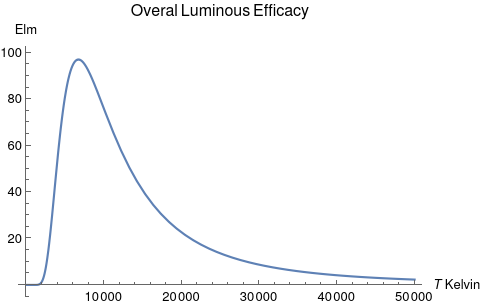
\includegraphics[width=\textwidth]{40_3.png}
    \caption{Problem 40.3: Plot of Efficacy vs. Temperature}
    \label{fig:40_3}
\end{figure}

\section*{41. The Simple and the Not-Quite-So-Simple Rigid Rotator}
A simple rigid rotator has only rotational energy, and its Hamiltonian is give by $ H = \frac{1}{2I} L^2 $ where $ L $ is the operator of angular momentum and $ I $ is the moment of inertia.
\begin{itemize}
    \item[1.] What are the eigenvalues of $ L $, and what are their degeneracies?
        \begin{problem}
            The eigenvalues of $ L $ are $ \hbar^2 l(l+1) $ and the degeneracies are $ g(l) \equiv 2l+1 $.
        \end{problem}
    \item[2.] Write down the canonical quantum partition function $ Z $ of the rigid rotator, as well as its free energy $ F $, energy $ U $, and specific heat $ c $. Substitute $ T_{\text{rot}} = \frac{\hbar^2}{2Ik_B} $.
        \begin{problem}
            \begin{equation}
                Z = \Tr[e^{- \beta H}] = \sum_{l=0}^{\infty} g(l) e^{- \beta l(l+1) \frac{\hbar^2}{2I}} =\sum_{l=0}^{\infty} g(l) e^{- \beta l(l+1) k_B T_{\text{rot}}}
            \end{equation}
            For convenience, I'll define $ \epsilon(l) \equiv l(l+1) k_B T_{\text{rot}} $.
            \begin{equation}
                F = - k_B T \log[Z] = -k_B T \log[\sum_{l=0}^{\infty} g(l) e^{- \beta \epsilon(l)}]
            \end{equation}
            \begin{equation}
                U = - \pdv{\beta} \log[Z] = \frac{\sum_{l=0}^{\infty} g(l) \epsilon(l) e^{- \beta \epsilon(l)}}{Z}
            \end{equation}
            \begin{align}
                c_V &= \pdv{T}U = - \pdv{T} \pdv{\beta} \log[Z] = \frac{(\partial_T Z)(\partial_{\beta} Z)}{Z^2} - \frac{\partial_T \partial_{\beta} Z}{Z} \\
                &= \frac{(\sum_{l=0}^{\infty} - g(l) \epsilon(l) e^{- \beta \epsilon(l)})(\sum_{l=0}^{\infty} k_B^{-1} T^{-2} g(l) \epsilon(l) e^{- \beta \epsilon(l)})}{Z^2} - \frac{\sum_{l=0}^{\infty} k_B^{-1} T^{-2} \epsilon(l)^2 g(l) e^{- \beta \epsilon(l)}}{Z}
            \end{align}
        \end{problem}
    \item[3.] Plot $ c(T) / k_B $ as a function of $ T/T_{\text{rot}} $ for $ 0 \leq T/T_{\text{rot}} \leq 3 $. Give an analytical explanation for the limit $ T \to \infty $.
        \begin{problem}
            All the plots are located at the end of this document. I did a partial sum up to about 40 because after that point, $ e^{l(l+1)} $ for $ l > 40 $ evaluates to basically zero in Mathematica, so I figured that around that order of magnitude would cancel out the other terms. Analytically, for large $ T $, all of the exponentials go to $ e^{0} = 1 $, so we get
            \begin{equation}
                Z = \sum g(l) 
            \end{equation}
            and
            \begin{equation}
                c_V = \frac{(\sum - g(l) \epsilon(l)) (\sum k_B^{-1} T^{-2} g(l) \epsilon(l))}{(\sum g(l))^2} - \frac{\sum k_B^{-1} T^{-2}\epsilon(l)^2 g(l)}{\sum g(l)} \to 0
            \end{equation}
            The factors of $ T^{-2} $ also go to $ 0 $, so in the end we just have a bunch of zeros, so I must have done something wrong when I calculated the derivatives, but I cant figure out what it would be (since the Mathematica answer makes it seem like it approaches $ 1 $).
        \end{problem}
    \item[4.] Repeat with parahydrogen.
        \begin{problem}
            I would rather not write everything out again, since, in my notation, all of the equations will be identical. Instead, I'll just explain that for parahydrogen, we are looking at the singlet state which must have $ l $ be even, so I can substitute $ l \to 2l $ in the equations for $ \epsilon(l) $ and $ g(l) $ above.
        \end{problem}
    \item[5.] Repeat for orthohydrogen.
        \begin{problem}
            Again, I won't write it out. There are three degenerate states which must have $ l $ odd, so $ g(l) \to 3g(2l+1) $ and $ \epsilon(l) \to \epsilon(2l+1) $.
        \end{problem}
    \item[6.] Repeat for the equilibrium state.
        \begin{problem}
            Here, we just want to include both ortho- and parahydrogen in the summations. Note that $ \frac{1 + (-1)^l}{2} = \begin{cases} 1 & l \text{ even} \\ 0 & l \text{ odd} \end{cases} $ acts as an indicator function for the parity of $ l $. With some simple manipulation, I can turn this into $ p(l) \equiv 2-(-1)^l $, which gives the desired degeneracy of $ 1 $ for parahydrogen and $ 3 $ for orthohydrogen, but only at those specific parities. The partition function then becomes
            \begin{equation}
                Z = \sum_{l=0}^{\infty} p(l) g(l) e^{- \beta \epsilon(l)}
            \end{equation}
            and the other equations are identical with a multiplication of $ p(l) $ after each sum.
        \end{problem}
    \item[7.] Repeat for normal hydrogen.
        \begin{problem}
            Normal hydrogen can be treated as two distinct gasses in a fixed ratio. The new heat capacity is
            \begin{equation}
                c_{\text{normal}} = \frac{1}{4} c_{\text{para}} + \frac{3}{4} c_{\text{ortho}} 
            \end{equation}
        \end{problem}
    \item[8.] Plot the four theoretically calculated rotational specific heats for $ 0 \leq T/T_{\text{rot}} \leq 3.5 $. By a careful comparison with the experimentally measured rotational specific heat, determine the length of the hydrogen-hydrogen bond.
        \begin{problem}
            The graph is attached. Experimentally (without units) I chose $ c = \{0.5, 0.75, 0.8\} $ for $ T = \{150\kelvin, 185\kelvin, 200\kelvin\} $ in the experimental plot. On my plot, I found the temperature values corresponding to those values of $ c $: $ T' = \{2.054, 9.3725, 9.3728\} $. By averaging, $ T_{\text{rot}} = \frac{1}{3} \sum \frac{T}{T'} \approx 38.0249 $. Recall that $ T_{\text{rot}} = \frac{\hbar^2}{2I k_B} $ and for a rigid rotator comprised of two fixed masses connected by a massless rod, $ I = \frac{mL^2}{2} $, so
            \begin{equation}
                L = \sqrt{\frac{\hbar^2}{k_B m T_{\text{rot}}}} = 1.12491\times 10^{-10} \meter \neq 74\pico\meter
            \end{equation}
            I must have some error in my calculation.
        \end{problem}
\end{itemize}
\begin{figure}[h]
    \centering
    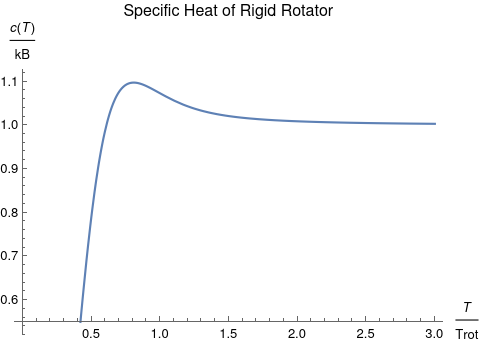
\includegraphics[width=\textwidth]{41_3.png}
    \caption{Plot for Problem 41.3}
    \label{fig:41_3}
\end{figure}
\begin{figure}[h]
    \centering
    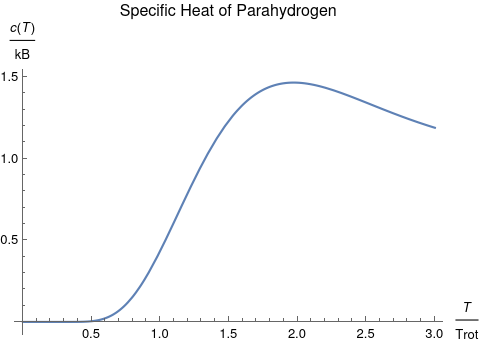
\includegraphics[width=\textwidth]{41_4.png}
    \caption{Plot for Problem 41.4}
    \label{fig:41_4}
\end{figure}
\begin{figure}[h]
    \centering
    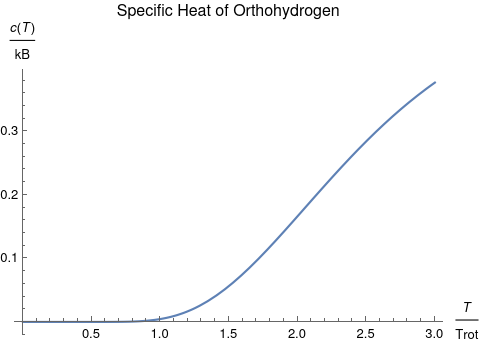
\includegraphics[width=\textwidth]{41_5.png}
    \caption{Plot for Problem 41.5}
    \label{fig:41_5}
\end{figure}
\begin{figure}[h]
    \centering
    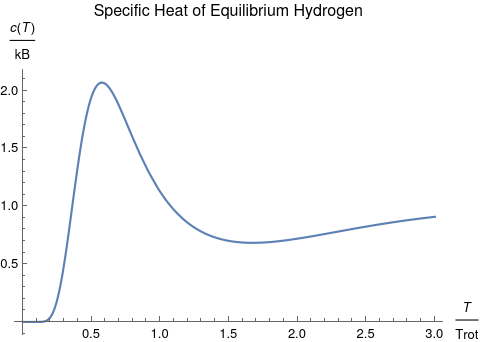
\includegraphics[width=\textwidth]{41_6.png}
    \caption{Plot for Problem 41.6}
    \label{fig:41_6}
\end{figure}
\begin{figure}[h]
    \centering
    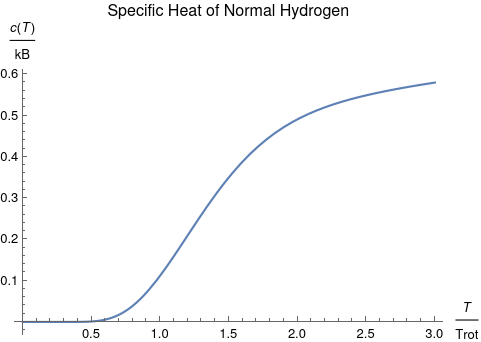
\includegraphics[width=\textwidth]{41_7.png}
    \caption{Plot for Problem 41.7}
    \label{fig:41_7}
\end{figure}
\begin{figure}[h]
    \centering
    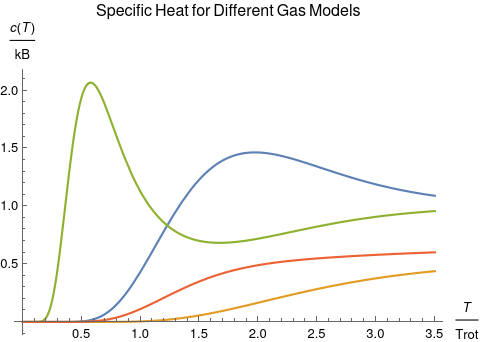
\includegraphics[width=\textwidth]{41_8.png}
    \caption{Plot for Problem 41.8}
    \label{fig:41_8}
\end{figure}



\end{document}
